\documentclass[../main/main.tex]{subfiles}
\begin{document}
\chapter{Superconducting qubits}

\section{Josephson junctions and Josephson effect} \label{sect:josephson_junction_effect}
In 1962 Brian David Josephson demonstrated theoretically that Cooper pairs can tunnel through a barrier generating a current \cite{JOSEPHSON1962251}. The tunneling of normal-conducting electrons was a well-known fact \cite{PhysRevLett.8.316,shapiro_5392409}, but the tunneling of an electron pair was never observed. One year after Josephson's paper, Anderson and Rowell claimed to have observed experimentally such an effect \cite{PhysRevLett.10.230}. \par
\begin{figure}[ht]
    \vspace{0.2cm}
    \centering
    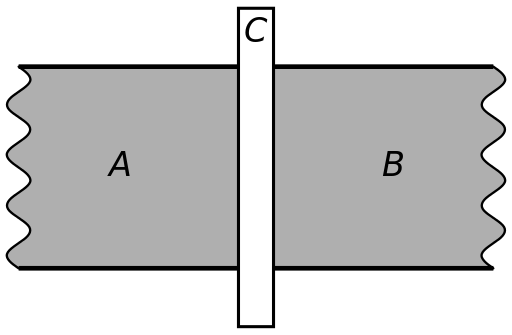
\includegraphics[width=0.45\textwidth]{../images/josephson_junction.png}
    \vspace{-0.2cm}
    \caption{Schematic of a Josephson junction. A,B are the superconductors and C is the insulating layer. From \url{https://commons.wikimedia.org/wiki/File:Single_josephson_junction.svg} [accessed 31 Aug, 2021].}
    \label{fig:josephson_junction}
\end{figure}
\vspace{0.4cm}
Josephson junctions are devices in which two or more superconductors are coupled by a thin layer of insulating material. By connecting the junction to an external circuit it is possible to measure both the current and the voltage drop across the barrier. The difficulties in observing the Josephson tunneling phenomenon are due to the strong influence that temperature and magnetic fields have on the Cooper pairs. \par
We now proceed with the demonstration of some of the effects observed in a Josephson junction using a simple model. Two superconductors of the same material are connected as in Fig.~\ref{fig:josephson_junction} and the temperature of the setup is well below the critical temperature $T_C$: the electrons are thus in the BCS ground state. According to the Ginzburg-Landau theory \cite{Landau:486430}, Cooper pairs can be described by a complex order parameter
\begin{equation} \label{eq:Psi_j_definition}
    \Psi_j=\sqrt{n_{cj}}\ e^{i \phi_j},
\end{equation}
in which $n_{cj}$ is the density of Cooper pairs in the superconductor indexed by $j=A,B$ as in Fig.~\ref{fig:josephson_junction}. The phases of the complex $\Psi$ can be different on the two sides of the junction because of the weakness of the link represented by the barrier. Given the Hamiltonians $\hat{H}_j$ of the isolated superconductor and the coupling constant $\mathcal{T}$ of the tunnel junction, $\Psi_j$ satisfy
\begin{align} \label{eq:tunnel_junction_evolution}
    i \hbar \frac{\partial \Psi_A}{\partial t} &= \hat{H}_A \Psi_A + \mathcal{T} \Psi_B , &
    i \hbar \frac{\partial \Psi_B}{\partial t} &= \hat{H}_B \Psi_B + \mathcal{T} \Psi_A .
\end{align}
We now suppose the $\Psi_j$ to be eigenstates of the Hamiltonians $\hat{H}_j$ and thus $\hat{H}_j \Psi_j = E^0_j \Psi_j$. Because of the symmetries of the model, $E^0_A = E^0_B \equiv E^0$ holds.\\
A voltage $U$ applied across the junction causes an energy shift $\Delta E = E_A - E_B = q\, U$ between the two superconductors, with $q=-2e$ being the Cooper pair charge. Defining as zero the midpoint energy of the two superconductors, Eq.~\eqref{eq:tunnel_junction_evolution} simplifies to
\begin{align} \label{eq:tunnel_junction_evolution2}
    i \hbar \frac{\partial \Psi_A}{\partial t} &= \frac{q\, U}{2} \Psi_A + \mathcal{T} \Psi_B , &
    i \hbar \frac{\partial \Psi_B}{\partial t} &= -\frac{q\, U}{2} \Psi_B + \mathcal{T} \Psi_A .
\end{align}
Inserting Eq.~\eqref{eq:Psi_j_definition} into Eq.~\eqref{eq:tunnel_junction_evolution2} and separating real parts and imaginary parts we get
\begin{align} \label{eq:solutions_Psi_j}
    \dot{n}_{cA} &= \frac{2\mathcal{T}}{\hbar} \sqrt{n_{cA} n_{cB}} \sin{(\phi_B-\phi_A)}, & 
    \dot{\phi}_A &= -\frac{\mathcal{T}}{\hbar} \sqrt{\frac{n_{cB}}{n_{cA}}} \cos{(\phi_B-\phi_A)} - \frac{q\, U}{2\hbar}, \\
    \dot{n}_{cB} &= -\frac{2\mathcal{T}}{\hbar} \sqrt{n_{cA} n_{cB}} \sin{(\phi_B-\phi_A)}, & 
    \dot{\phi}_B &= -\frac{\mathcal{T}}{\hbar} \sqrt{\frac{n_{cA}}{n_{cB}}} \cos{(\phi_B-\phi_A)} + \frac{q\, U}{2\hbar} . \nonumber
\end{align}
Assuming $n_{cA} = n_{cB} \equiv n_c$ for symmetry considerations and defining the difference of wave function phases as $\delta = \phi_B-\phi_A$, Eq.~\eqref{eq:solutions_Psi_j} leads to
\begin{align} \label{eq:solutions2_Psi_j}
    \dot{n}_{cA} + \dot{n}_{cB} &= 0, & 
    \dot{\delta} = \dot{\phi}_B - \dot{\phi}_A &= \frac{q\, U}{\hbar}.
\end{align}
The first result of Eq.~\eqref{eq:solutions2_Psi_j}
confirms the conservation of the total number of Cooper pairs in the two superconductors, while the second result gives information about the oscillation of the quantities in Eq.~\eqref{eq:solutions_Psi_j}, namely
\begin{equation} \label{eq:delta_time_integration}
    \delta(t) = \delta_0 + \frac{q}{\hbar} \int_{0}^{t} U(\nu) \,d\nu ,
\end{equation}
where $\delta_0$ is the difference of the wave function phases at the initial time $t=0$. We are interested in the case of a constant voltage $U$, thus the equation of the tunnel current has the form
\begin{equation} \label{eq:tunnel_current_J}
    J_{\mathcal{T}}(t) = \frac{2 \mathcal{T} n_c}{\hbar} \sin{\left(\delta_0 - \frac{2e U}{\hbar}t\right)} = J_0 \sin{\left(\delta_0 - \frac{2e U}{\hbar}t\right)}.
\end{equation}
Equation~\eqref{eq:tunnel_current_J} summarizes the conclusions made by Josephson in his 1962 paper \cite{JOSEPHSON1962251}. For finite voltages $U$, an alternating supercurrent occurs. That current has an amplitude of $J_0 = 2 \mathcal{T} n_c/\hbar$ and a frequency of $f=2 e U /(2\pi \hbar) = 2 e U/h$. Instead, for a vanishing voltage $(U=0)$ a direct current up to a maximum of $J_0$ occurs. The direction of this DC current and its magnitude depend on the value of $\delta_0$.
\section{Charge qubits} \label{sect:charge_qubits}
As seen in the previous section, below the critical temperature Josephson junctions allow the tunneling of Cooper pairs across the barrier. This process is dissipationless and maintains the coherence of the Cooper pair states under suitable conditions (e.g., low temperatures, external fields screening, etc.). Also, Josephson junctions can be embedded in electronic circuits and coupled with other Josephson junctions. Such properties suggest Josephson junctions as possible quantum devices to be used as \textit{qubits}. \par
\begin{figure}[ht]
    \vspace{-0.1cm}
    \centering
    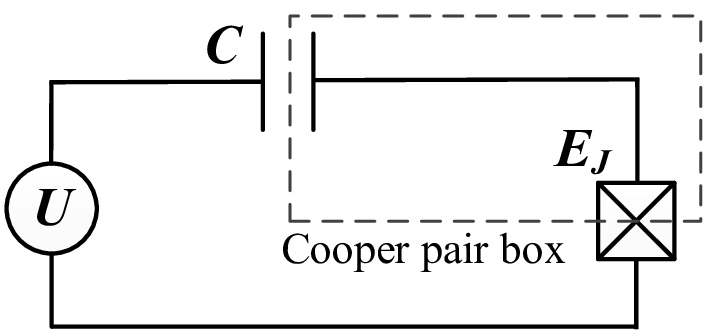
\includegraphics[width=0.5\textwidth]{../images/charge_qubit.png}
    \vspace{-0.2cm}
    \caption{Schematic representation of a charge qubit. $E_J$ is the Josephson energy, $U$ is the gate voltage and $C$ is the gate capacitance. The dashed rectangle represents the box with the excess of Cooper pairs \cite[Figure~2]{Wu_Nori_2012}.}
    \label{fig:charge_qubit}
\end{figure}
In quantum computing, a qubit is a two-level quantum system that represents the basic unit of quantum information. The qubit can be in the states $\ket{0}$, $\ket{1}$ or even in a coherent superposition of these two states, according to quantum mechanics. The manipulation of the qubit state is provided by the \textit{qubit gates}. The implementation of these qubit gates depends on the setup chosen to represent the qubit. For instance, in Josephson junctions the necessary gates can be obtained by controlling applied voltages, magnetic fields and the coupling with other Josephson junctions. \par
We now focus on the specific setup of charge qubits \cite{RevModPhys.73.357}. A charge qubit consists of a small superconducting island (the "box" in Fig.~\ref{fig:charge_qubit}) connected by a thin insulator to a superconducting reservoir. Cooper pairs can tunnel through the insulator by the Josephson effect. The number $n$ of excess Cooper pairs in the box, relatively to some reference state, is the degree of freedom of the system. The proper choice of the experimental parameters allows to restrict $n$ to a set of only two values, transforming the junction to a two-level quantum system, i.e., a qubit.\\
The tunnel junction has capacitance $C_J$, Josephson coupling energy $E_J$, and it is biased by an external controllable voltage $U$ with gate capacitance $C$. The voltage $U$ has the same role of the voltage of Sect.~\ref{sect:josephson_junction_effect}. In the arrangement of charge qubits, the charging energy of an electron is \mbox{$E_C = e^2/2 \, (C+C_J)$} and $E_J$ is related to the maximum current that can flow through the tunnel junction without dissipation. In low-capacitance charge qubits the charging energy is greater than the Josephson energy by a factor of 10. Using junctions with capacitances $C_J \leq 10^{-15}\,$F and gates with even smaller capacitances, charging energy is in the range $E_C/k_B \geq 1\,$K and consequently $E_J/k_B \sim 100\,$mK. The superconducting material is the same on both sides and the energy gap $\Delta$ is larger than every characteristic energy of the system. At low temperatures the single-electron tunneling is exponentially suppressed, because an unpaired electron would cost an additional energy of $\Delta$ to the ground state energy. Under such conditions, only Cooper pairs tunnel through the barrier, and they tunnel coherently. The system is described by the Hamiltonian \cite{RevModPhys.73.357,benenti_casati_strini_quantum_computation_information}
\begin{equation} \label{eq:Hamiltonian_charge_qubits}
    \hat{H}_{1Q} = 4 E_C\, (\hat{n}-n_g)^2 - E_J\, \cos{\hat{\Theta}},
\end{equation}
in which $\hat{n}$ is the number operator of excess Cooper-pair charges on the box and $\hat{\Theta}$ is the phase of the superconducting order parameter of the box. Operators $\hat{n}$ and $\hat{\Theta}$ are canonically conjugate, so $[\hat{\Theta},\hat{n}]=i$ holds. The dimensionless gate charge $n_g = C U / 2 e$ can be controlled by tuning the value of the gate voltage $U$. For $E_C \gg E_J$ the Hamiltonian~\eqref{eq:Hamiltonian_charge_qubits} can be conveniently written in the basis of eigenstates $\ket{n}$ of the number operator $\hat{n}$. The $\cos{\hat{\Theta}}$ term in this basis evaluates as
\begin{equation} \label{eq:cosTheta_n_basis}
    \cos{\hat{\Theta}} \ket{n} = \frac{1}{2} \left( e^{i \hat{\Theta}} + e^{-i \hat{\Theta}} \right) \ket{n} =  \frac{1}{2} \left( \ket{n+1} + \ket{n-1} \right).
\end{equation}
Hence, the Hamiltonian~\eqref{eq:Hamiltonian_charge_qubits} in the $\ket{n}$-basis reads as
\begin{equation} \label{eq:Hamiltonian_charge_qubits_ket_n_basis}
    \hat{H}_{1Q} = \sum_n \left[ 4 E_C\, (n-n_g)^2 \ket{n}\!\bra{n} - \frac{1}{2} E_J \left( \ket{n+1}\!\bra{n} + \ket{n}\!\bra{n+1} \right) \right].
\end{equation}
The Hamiltonian~\eqref{eq:Hamiltonian_charge_qubits_ket_n_basis} is, with good approximation, diagonal in the $\ket{n}$-basis for almost every value of $n_g$ because $E_C \gg E_J$. Thus, the charge states $\ket{n}$ are weakly mixed by the $E_J$-term. An important exception is the case of half-integer $n_g$. Indeed, if $n_g$ is half-integer the charging energies of the two states $\ket{n_g-\frac{1}{2}}$ and $\ket{n_g+\frac{1}{2}}$ are equal and the $E_J$-term mixes strongly the two states. At low temperatures ($T \ll E_C/k_B$) the dynamic of the system is limited to these two states. We assume $n_g \in [0,1]$ in the following calculations. The Hamiltonian~\eqref{eq:Hamiltonian_charge_qubits_ket_n_basis}, written in spin-$1/2$ notation and restricted to the states $\ket{0},\ket{1}$, simplifies to
\begin{equation} \label{eq:Hamiltonian_charge_qubits_halfspin}
    \hat{H}_{1Q} = -\frac{1}{2} B_z \hat{\sigma}_z -\frac{1}{2} B_x \hat{\sigma}_x,
\end{equation}
in which we defined
\begin{align} \label{eq:matrices_definition}
    \ket{0} &= 
    {\begin{pmatrix}
    1 \\ 0
    \end{pmatrix}},
    &
    \hat{\sigma}_z &= 
    {\begin{pmatrix}
    1 & 0 \\ 0 & -1
    \end{pmatrix}},
    &
    B_z &= 4 E_C (1 - 2 n_g),
    \\
    \ket{1} &= 
    {\begin{pmatrix}
    0 \\ 1
    \end{pmatrix}},
    &
    \hat{\sigma}_x &= 
    {\begin{pmatrix}
    0 & 1 \\ 1 & 0
    \end{pmatrix}},
    &
    B_x &= E_J.
    \nonumber
\end{align}
The spin-$1/2$ notation has the quality of describing any two-state quantum system with an Hamiltonian $\hat{H}(t)=-\frac{1}{2} \boldsymbol{B}(t) \cdot \boldsymbol{\hat{\sigma}}$, where $\hat{\sigma}_{x,y,z}$ are Pauli matrices. The implementation of charge qubits allows to tune the $\hat{\sigma}_z$-term of $\hat{H}_{1Q}$ by controlling the gate voltage $U$, while the $\hat{\sigma}_x$-term is fixed by the value of Josephson charging energy $E_J$. However, a setup that uses two Josephson junctions in a loop configuration allows the tuning of $E_J$ by controlling an external flux $\Phi_x$ in the center of the loop \cite[Sect.~IIB]{RevModPhys.73.357}. By controlling both $B_x$ and $B_z$ it is possible to implement all of the one-qubit logic gates. \par
In order to obtain two-qubit logic gates we need to couple qubits in pairs and to control the interactions between them. This operation can be achieved by connecting with a capacitor the superconducting boxes of two qubits\footnote{Although leading to easy theoretical calculations, the switches used in the implementation of this qubit interaction introduce strong dephasing effects. So, different types of coupling are usually used in the experiments.}. The resulting charge-charge interaction can be described by a $\hat{\sigma}_z^1 \hat{\sigma}_z^2$-term in the Hamiltonian. With a controlled inter-qubit interaction of this type, we will see in Sect.~\ref{sect:implementation_qubit_gates} that it is possible to realize easily the controlled-NOT gate. The Hamiltonian of two coupled qubits is thus
\begin{equation} \label{eq:Hamiltonian_2_charge_qubits_halfspin}
    \hat{H}_{2Q} = -\frac{1}{2} B_z^1 \hat{\sigma}_z^1 -\frac{1}{2} B_x^1 \hat{\sigma}_x^1 -\frac{1}{2} B_z^2 \hat{\sigma}_z^2 -\frac{1}{2} B_x^2 \hat{\sigma}_x^2 + E_{CC}\, \hat{\sigma}_z^1 \hat{\sigma}_z^2 .
\end{equation}
The parameter $E_{CC}$ represents the tunable Coulomb charging energy associated to the qubits. The ability to tune $B_x^{1,2},\,B_z^{1,2},\,E_{CC}$ allows us to implement a universal set of gates.
\section{Implementation of qubit gates} \label{sect:implementation_qubit_gates}
Here we show how to obtain the logic gates by tuning properly the charge qubit controls. The gates' symbols are defined without the hat to improve readability.
\subsection{One-qubit gates} \label{sect:1Q_gates_implementation}
Using Eq.~\eqref{eq:Hamiltonian_charge_qubits_halfspin} we can calculate the one-qubit time-evolution operator 
\begin{equation} \label{eq:time_evolution_H1Q}
    \hat{\mathcal{U}}_{1Q}(\tau) = \exp{\left(-\frac{i \tau}{\hbar} \hat{H}_{1Q}\right)} = {\begin{pmatrix}
    \cos \frac{\tau \mathcal{B}}{2\hbar}+i\frac{B_z}{\mathcal{B}} \sin \frac{\tau \mathcal{B}}{2\hbar}
    & 
    i\frac{B_x}{\mathcal{B}} \sin \frac{\tau \mathcal{B}}{2\hbar}
    \\
    i\frac{B_x}{\mathcal{B}} \sin \frac{\tau \mathcal{B}}{2\hbar}
    &
    \cos \frac{\tau \mathcal{B}}{2\hbar}-i\frac{B_z}{\mathcal{B}} \sin \frac{\tau \mathcal{B}}{2\hbar}
    \end{pmatrix}},
\end{equation}
in which we defined $\mathcal{B} = \sqrt{(B_x)^2 + (B_z)^2}$. This operator represents the most general one-qubit gate that can be obtained by a quantum state evolution of time $\tau$ when the charge-qubit parameters $n_g$ and $E_J$ are fixed. \par
A rotation of angle $\alpha$ around the x-axis is described by the matrix
\begin{equation} \label{eq:alpha_x_axis_rotation}
    U_x(\alpha) = {\begin{pmatrix}
    \cos \frac{\alpha}{2} 
    &
    i \sin \frac{\alpha}{2}
    \\
    i \sin \frac{\alpha}{2}
    &
    \cos \frac{\alpha}{2} 
    \end{pmatrix}},
\end{equation}
and it can be obtained from Eq.~\eqref{eq:time_evolution_H1Q} by setting $B_z = 0$. This result can be achieved in the simplest implementation of charge qubits by setting $n_g = 1/2$, i.e., by switching on an external voltage $U=e/C$, for a timespan of $\tau$. The Josephson energy $E_J$ is fixed under such assumption. To obtain the desired $\alpha$-rotation the time of evolution has to be set to $\tau=\hbar \alpha / E_J$ if $E_J>0$. Typical timespans of this implementation are in the range of $0.1\,$ns for $E_J/k_B \sim 100\,$mK. \par
A z-rotation of angle $\beta$ is instead described by
\begin{equation} \label{eq:alpha_z_axis_rotation}
    U_z(\beta) = {\begin{pmatrix}
    e^{ i \beta/2 }
    &
    0
    \\
    0
    &
    e^{ -i \beta/2 }
    \end{pmatrix}},
\end{equation}
and the corresponding qubit gate is obtained by setting $B_x=0$ in the time evolution operator $\hat{\mathcal{U}}_{1Q}(\tau)$. It is possible to approximately implement such gate in charge qubits since $E_C \gg E_J$. The gate voltage $U$ could be, for instance, set at 0, so that also $n_g=0$ and $B_z=4 E_C \gg E_J = B_x$ holds. The rotation of an angle $\beta$ around the z-axis is then achieved by setting $\tau=\hbar \beta/(4 E_C)$. For $E_C/k_B \geq 1\,$K this implementation has typical timespans of $\tau \lesssim 1\,$ps. With a more complicated setup $B_x=0$ can be achieved by tuning exactly $E_J=0$. \par
Using combinations of x- and z-rotations, it is possible to obtain all the one-qubit gates. The NOT gate
\begin{equation} \label{eq:NOT_gate}
    \text{NOT} = {\begin{pmatrix}
    0
    &
    1
    \\
    1
    &
    0
    \end{pmatrix}},
\end{equation}
is equivalent to a $\pi$-rotation around the x-axis up to a global phase factor of $i$. While the Hadamard gate
\begin{equation} \label{eq:Hadamard_gate}
    H = \frac{1}{\sqrt{2}}{\begin{pmatrix}
    1
    &
    1
    \\
    1
    &
    -1
    \end{pmatrix}},
\end{equation}
needs three rotations if $B_x$ and $B_z$ cannot be switched on simultaneously, as it is the case of the simple charge qubit implementation. Indeed,
\begin{equation} \label{eq:Hadamard_gate_xz_rotation_implementation}
    H \propto U_x(\pi/4)\, U_z(\pi/4)\, U_x(\pi/4).
\end{equation}
The ability to simultaneously switch $B_x=B_z$ for a time $\tau=\hbar \pi/B_x$ allows an easier and faster implementation of the Hadamard gate. In the charge qubit setup these controls can be achieved by fixing a value of $E_J$ and by setting the external voltage $U$ so that $n_g = \frac{1}{2}-\frac{E_J}{8 E_C}$. The time of evolution is thus $\tau = \hbar \pi/E_J$ in this implementation.
\subsection{Two-qubit gates} \label{sect:2Q_gates_implementation}
The two-qubit time-evolution operator is defined similarly as
\begin{equation} \label{eq:time_evolution_H2Q}
    \hat{\mathcal{U}}_{2Q}(\tau) = \exp{\left(-\frac{i \tau}{\hbar} \hat{H}_{2Q}\right)},
\end{equation}
but the characterization of its general form is outside of the scope of this thesis. Indeed, the CNOT gate is the only two-qubit gate we are interested in, since the other two-qubit gates can be obtained with only one-qubit operations. The $\hat{\sigma}_z^1 \hat{\sigma}_z^2$-coupling of the Hamiltonian~\eqref{eq:Hamiltonian_2_charge_qubits_halfspin} allows the implementation of CNOT gate with only a two-qubit operation \cite[Appx.~B3]{RevModPhys.73.357}, 
\begin{equation} \label{eq:CNOT_gate}
   \text{CNOT} \propto H^2\ \left[U_z^1(-\pi/2)\ U_z^2(-\pi/2)\ \exp{\left(i\frac{\pi}{4} \hat{\sigma}_z^1 \hat{\sigma}_z^2 \right)}\right]\ H^2,
\end{equation}
in which $H^2$ is the Hadamard gate applied to the qubit 2. Supposing we have a system in which the Coulomb charging energy $E_{CC}$ is negative, the $\exp{\left(i\frac{\pi}{4} \hat{\sigma}_z^1 \hat{\sigma}_z^2 \right)}$-term in the CNOT implementation can be obtained by tuning the inter-qubit coupling for a timespan $\tau=\hbar \pi /(4 |E_{CC}|)$ while setting $E_J=0$ and $n_g=0$ for both qubits.
\end{document}
